\documentclass[pdf]{beamer}
\mode<presentation>{} 



\usepackage{hyperref}
\usepackage{pgf}
\usepackage{fancyhdr}
\usepackage{tikz}
\usetikzlibrary{trees}
\usetikzlibrary{arrows,automata}
\usetikzlibrary{automata,positioning}
\usetikzlibrary{shapes}
\usepackage{tikz-qtree,tikz-qtree-compat}
\usepackage{mathtools,enumerate,amssymb}
\usetikzlibrary{patterns}
\usepackage[utf8]{inputenc}
\usepackage[T1]{fontenc}
\usepackage{graphicx}
\usepackage{varwidth}
\usepackage{xcolor}
\usepackage{multicol}
\usepackage{multirow}
\usepackage[export]{adjustbox}
\usepackage{wrapfig}
\usepackage{textcomp}
\usepackage{eso-pic}
\usepackage{pgfornament}
\usepackage[export]{adjustbox}
\usepackage{longtable}



\title{Visual Variables}
\subtitle{Human Computer Interaction}
\AtBeginSection[]{}



\definecolor{background}{RGB}{255,255,255}
\setbeamercolor{background canvas}{bg=background}
\setbeamercolor{frametitle}{fg=blue}



\setbeamertemplate{sidebar right}{}
\setbeamertemplate{footline}{%
\hfill\usebeamertemplate***{navigation symbols}
\hspace{1cm}\insertframenumber{}/\inserttotalframenumber}

\graphicspath{{./img/}}



\begin{document}



{\setbeamercolor{background canvas}{bg=background}
\begin{frame}
\vspace{10mm}
\huge{\raggedleft{\color{black}{\textbf{Visual Variables}}}}

\large{\raggedleft{\color{black} Human Computer Interaction}}

\begin{flushright}
\end{flushright}

\fontsize{7pt}{1pt}\selectfont{
Based on slide deck 

\textbf{Part 4: Designing and building visual interfaces. Visual Variables}

Human Computer Interaction I: Principles and Design

by

\textbf{Saul Greenberg}
\newline
Professor
\newline
\textbf{University of Calgary, Canada}

\textit{The new slides are marked with a *}
}

\fontsize{5pt}{1pt}\selectfont{ \textcolor{lightgray}
{Slide deck by Saul Greenberg. Permission is granted to use this for non-commercial purposes as long as general credit to Saul Greenberg is clearly maintained.
Warning: some material in this deck is used from other sources without permission. Credit to the original source is given if it is known.}}

\end{frame}}



\definecolor{bluetext}{RGB}{0,0,102}
\definecolor{background}{RGB}{255,255,255}
\setbeamercolor{background canvas}{bg=background}
\begin{frame}
	\bigskip
    \textbf{\LARGE Visual Variables \LARGE}
   	\newline
    \newline
    \newline
    \textbf{Attributes of visual symbols}
    \newline
    \textbf{Characteristics of the attributes of visual symbols}
    \newline
    \textbf{How we distinguish between them}
    \newline
\end{frame}



% Inaintea codului fiecarui slide se vor scrie urmatoarele informatii:
% Nume si prenume student
% Numarul slide-ului corespunzator din prezentarea prof. Saul Greenberg
% Numele imaginilor inserate trebuie sa fie numar_slide_nume_imagine.extensie_imagine



%Dedita Vlad 
%2
\definecolor{textalbastru}{RGB}{0,0,102}
\definecolor{fundal}{RGB}{255,255,255}
\setbeamercolor{background canvas}{bg=fundal}
\begin{frame}
{\textbf{Visual variables - attributes}}{\textcolor{red}{\rule{12cm}{1.2pt}}}

     \begin{itemize}   
     	\item[]\hspace{-15px}\textbf{{{position}}}             	   	
        \item[--]{\small{changes in the x, y (z) location}}   	


\includegraphics[scale=0.45]{2_Imagine1.png}
                  
        \item[]\hspace{-15px}\textbf{{size}}     	
        \item[--]{\small{change in length, area or repetition}}   


\includegraphics[scale=0.4]{2_Imagine2.png}

\includegraphics[scale=0.4]{2_Imagine3.png}              
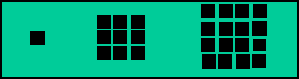
\includegraphics[scale=0.4]{2_Imagine4.png}               
        
     	\item[]\hspace{-15px}\textbf{{shape}}     	
        \item[--]{\small{infinite number of shapes}}      


\includegraphics[scale=0.45]{2_Imagine5.png}   
        
     	\item[]\hspace{-15px}\textbf{{value}}     	
        \item[--]{\small{changes from light to dark}}         


\includegraphics[scale=0.45]{2_Imagine6.png}   
        
     \end{itemize}

\end{frame}



\definecolor{textalbastru}{RGB}{0,0,102}
\definecolor{fundal}{RGB}{255,255,255}
\setbeamercolor{background canvas}{bg=fundal}
\begin{frame}
{\textbf{Visual variables - attributes}}{\textcolor{red}{\rule{12cm}{1.2pt}}}

     \begin{itemize}           
     	\item[]\hspace{-15px}\textbf{{orientation}}     	
        \item[--]{\small{changes in alignment}}       
        
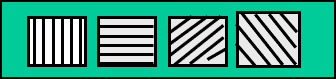
\includegraphics[scale=0.45]{2_Imagine7.png}     
        
     	\item[]\hspace{-15px}\textbf{{colour}}     	
        \item[--]{\small{changes in hue at a given value}} 

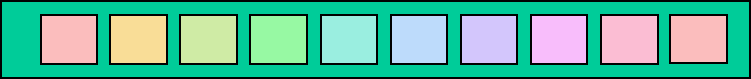
\includegraphics[scale=0.45]{2_Imagine8.png}     
               
     	\item[]\hspace{-15px}\textbf{{texture}}     	
        \item[--]{\small{variation in pattern}}        

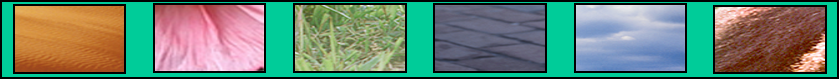
\includegraphics[scale=0.45]{2_Imagine9.png}   
        
        \item[]\hspace{-15px}\textbf{{motion}}    
        
     \end{itemize}

\end{frame}



%Dedita Vlad
%3
\begin{frame}
{\textbf{Visual variables - characteristics}}{\textcolor{red}{\rule{12cm}{1.2pt}}}

     \begin{itemize}
     	\item[--]\textbf{{{selective}}}
        \item[]\hspace{10px}{\small{is a change enough to allow us to select it from a group?}} 
        
     	\item[--]\textbf{{{associative}}}
        \item[]\hspace{10px}{\small{is a change enough to allow us to perceive them as a group?}}  
        
     	\item[--]\textbf{{{quantitative}}}
        \item[]\hspace{10px}{\small{is there a numerical reading obtainable from changes in this variable?}}  
     	\item[--]\textbf{{{order}}}
        \item[]\hspace{10px}{\small{are changes in this variable perceived as ordered?}}  
        
     	\item[--]\textbf{{{length}}}
        \item[]\hspace{10px}{\small{across how many changes in this variable are distinctions perceptible?}}          
      \end{itemize}     
      
\end{frame}



%Dedita Vlad
%4
\begin{frame}
{\textbf{Position}}{\textcolor{red}{\rule{12cm}{1.2pt}}}

\vspace{-1cm}

    \begin{minipage}{0.3\textwidth}
    \vspace{20px}
    \begin{itemize}
    		\setlength\itemsep{1.3em}
     		\item[\checkmark]\textbf{{{selective}}}
            \item[\checkmark]\textbf{{{associative}}}
            \item[\checkmark]\textbf{{{quantitative}}}
            \item[\checkmark]\textbf{{{order}}}
            \item[\checkmark]\textbf{{{length}}}
     \end{itemize}
  	\end{minipage}%
    \begin{minipage}{0.7\textwidth}
  	   \begin{picture}(0,0)
         \put(0,36){\hbox{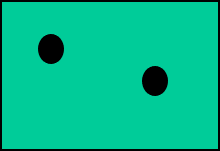
\includegraphics[scale=0.4]{4_Imagine1.png}}}
         \put(50,36){\hbox{
\includegraphics[scale=0.4]{4_Imagine2.png}}}
         \put(100,36){\hbox{
\includegraphics[scale=0.4]{4_Imagine3.png}}}
         \put(0,4){\hbox{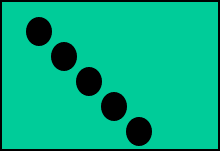
\includegraphics[scale=0.4]{4_Imagine4.png}}}
         \put(50,4){\hbox{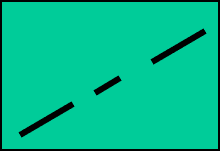
\includegraphics[scale=0.4]{4_Imagine5.png}}}
         \put(100,4){\hbox{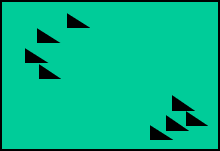
\includegraphics[scale=0.4]{4_Imagine6.png}}}
         \put(0,-115){\hbox{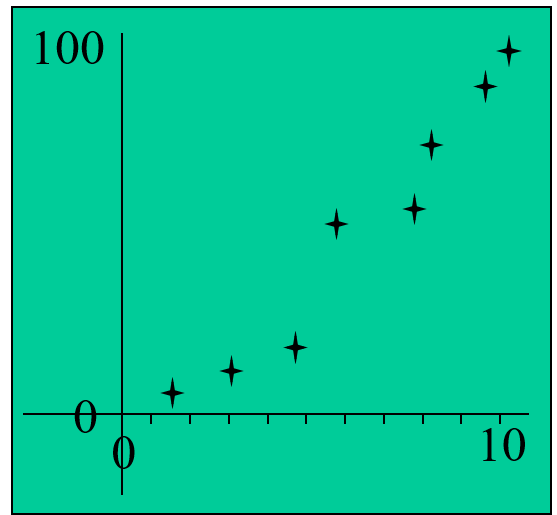
\includegraphics[scale=0.45]{4_Imagine7.png}}}
         
       \end{picture}
	\end{minipage}%
\end{frame}



%Dedita Vlad
%5
\begin{frame}
{\textbf{Size}}{\textcolor{red}{\rule{12cm}{1.2pt}}}
    
\vspace{1cm}    
    
    \begin{itemize}
    		\setlength\itemsep{1.6em}
           
     		\item[\checkmark]\textbf{{{selective}}}
            
            \item[\checkmark]\textbf{{{associative}}}
           
            \item[$\simeq$]\textbf{{{quantitative}}}
          	
            \item[\checkmark]\textbf{{{order}}}
            
            \item[\checkmark]\textbf{{{length}}}
            
            \begin{itemize}
             \item[--]\hspace{10px}{\small{theoretically infinite but practically limited}}  
             \item[--]\hspace{10px}{\small{association and selection $\sim$ 5 and distinction $\sim$ 20}}  
            \end{itemize}
     \end{itemize}
  
   
  	   \begin{picture}(0,0)
         \put(105,180){\hbox{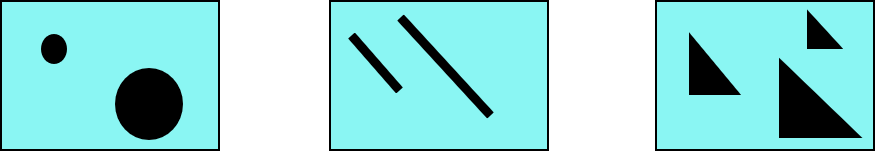
\includegraphics[scale=0.45]{5_Imagine1.png}}}
        
         \put(105,145){\hbox{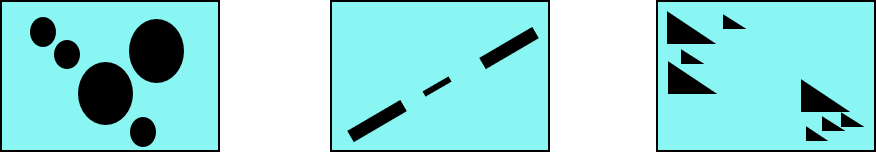
\includegraphics[scale=0.45]{5_Imagine2.png}}}
        
         \put(105,105){\hbox{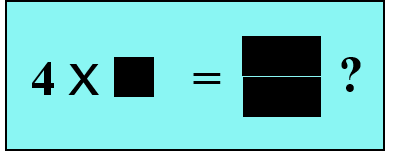
\includegraphics[scale=0.45]{5_Imagine3.png}}}
         
         \put(105,65){\hbox{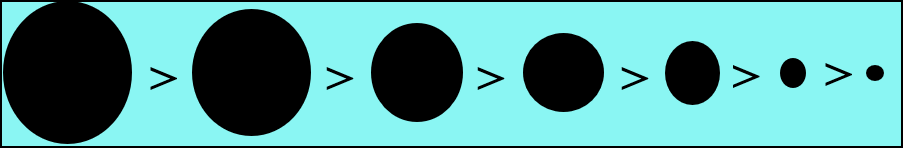
\includegraphics[scale=0.45]{5_Imagine4.png}}}
         
       \end{picture}
	
\end{frame}



%Dedita Vlad
%6
\begin{frame}
{\textbf{Shape}}{\textcolor{red}{\rule{12cm}{1.2pt}}}

    \begin{itemize}
    		\setlength\itemsep{1.6em}
           
     		\item[$\simeq$]\textbf{{{selective}}}
            
            \item[$\simeq$]\textbf{{{associative}}}
           
            \item[$\neq$]\textbf{{{quantitative}}}
          	
            \item[$\neq$]\textbf{{{order}}}
            
            \item[\checkmark]\textbf{{{length - infinite variation}}}
     \end{itemize}
     
  	   \begin{picture}(0,0)
         \put(105,140){\hbox{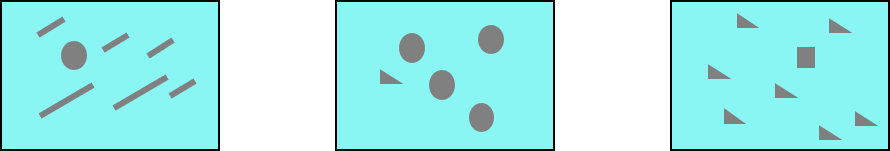
\includegraphics[scale=0.45]{6_Imagine1.png}}}
        
         \put(105,100){\hbox{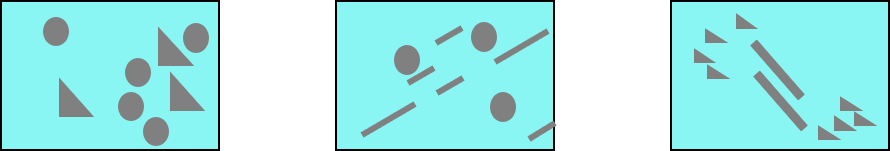
\includegraphics[scale=0.45]{6_Imagine2.png}}}
        
         \put(105,40){\hbox{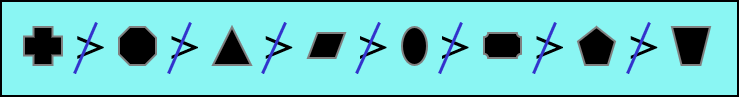
\includegraphics[scale=0.45]{6_Imagine3.png}}}
         
         \put(50,-10){\hbox{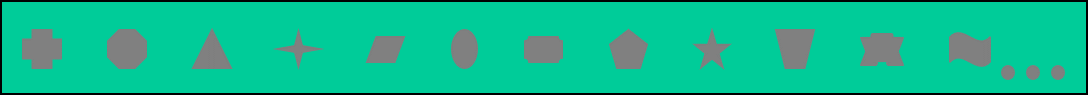
\includegraphics[scale=0.45]{6_Imagine4.png}}}
         
       \end{picture}
	
\end{frame}



%Dedita Vlad
%7
\begin{frame}
{\textbf{Shape}}{\textcolor{red}{\rule{12cm}{1.2pt}}}

\vspace{-4cm}
    
     \begin{picture}(0,0)
         \put(40,-80){\hbox{
\includegraphics[scale=0.5]{7_Imagine1.png}}}  
         \put(80,-150){\hbox{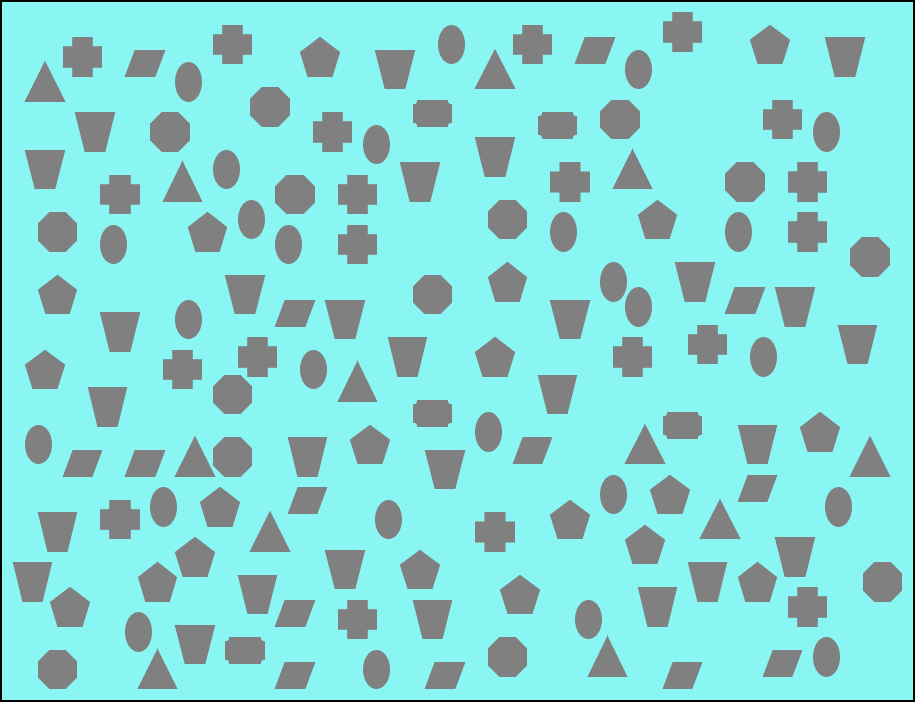
\includegraphics[scale=0.45]{7_Imagine2.png}}}  
         
       \end{picture}
	
\end{frame}



%Fer Andrei
%8
\definecolor{textalbastru}{RGB}{0,0,102}
\definecolor{fundal}{RGB}{255,255,255}
\setbeamercolor{background canvas}{bg=fundal}
\begin{frame}
{\textbf{Value}}{\textcolor{red}{\rule{12cm}{1.2pt}}}

\vspace{1cm}

     \begin{itemize}
       \item[\checkmark]\textbf{{{selective}}}
       \newline
       \newline
       \item[\checkmark]\textbf{{{associative}}}
       \newline
       \newline
       \item[$\neq$]\textbf{{{quantitative}}}
       \newline
       \item[\checkmark]\textbf{{{order}}}
       \newline
       \item[\checkmark]\textbf{{{length}}}
       
      \begin{itemize}
       \item[--]{theoretically infinite but practically limited}
       \item[--]{association and selection $\sim$ < 7 and distinction $\sim$ 10}
      \end{itemize}
     \end{itemize}
     
     \vspace{100px}
     
    \begin{picture}(0,0)
     \put(110,270){\hbox{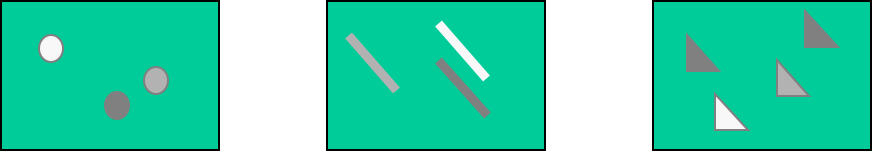
\includegraphics[scale=0.45]{8_Picture1.png}}}
     \put(110,225){\hbox{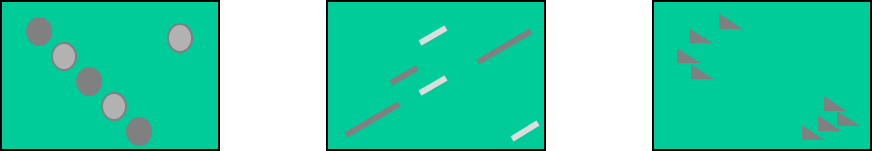
\includegraphics[scale=0.45]{8_Picture2.png}}}
     \put(110,190){\hbox{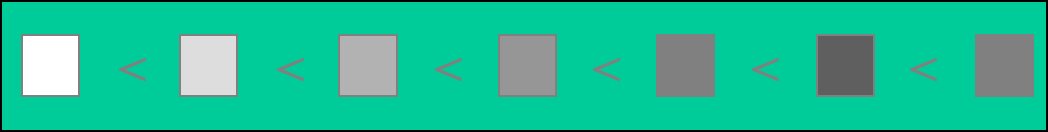
\includegraphics[scale=0.35]{8_Picture3.png}}}
    \end{picture}       
\end{frame}



%Fer Andrei
%9
\definecolor{textalbastru}{RGB}{0,0,102}
\definecolor{fundal}{RGB}{255,255,255}
\setbeamercolor{background canvas}{bg=fundal}
\begin{frame}
{\textbf{Color}}{\textcolor{red}{\rule{12cm}{1.2pt}}}

\vspace{1cm}

     \begin{itemize}
      \item[\checkmark]\textbf{{{selective}}}
      \newline
      \newline
      \item[\checkmark]\textbf{{{associative}}}
      \newline
      \item[$\neq$]\textbf{{{quantitative}}}
      \newline
      \item[$\neq$]\textbf{{{order}}}
      \newline
      \item[\checkmark]\textbf{{{length}}}
      \begin{itemize}
       \item[--]{theoretically infinite but practically limited}
       \item[--]{association and selection  $\sim$ < 7 and distinction $\sim$ 20}
      \end{itemize}
     \end{itemize}
     
     \vspace{100px}
     
    \begin{picture}(0,0)
     \put(110,255){\hbox{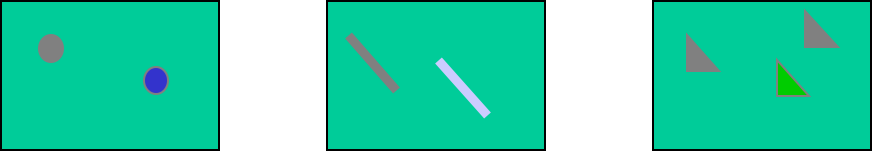
\includegraphics[scale=0.45]{9_Picture1.png}}}
     \put(110,210){\hbox{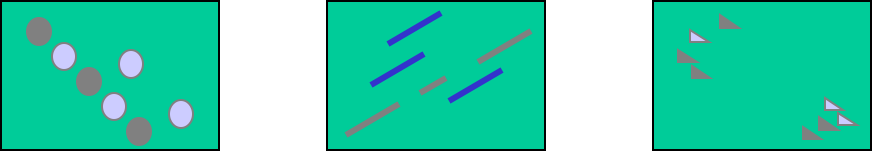
\includegraphics[scale=0.45]{9_Picture2.png}}}
     \put(110,160){\hbox{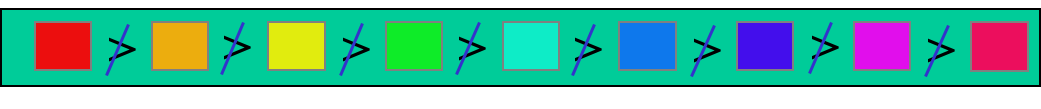
\includegraphics[scale=0.35]{9_Picture3.png}}}
     \put(0,100){\hbox{
\includegraphics[scale=0.45]{9_Picture4.png}}}
    \end{picture}       
\end{frame}



%Fer Andrei
%10
\definecolor{textalbastru}{RGB}{0,0,102}
\definecolor{fundal}{RGB}{255,255,255}
\setbeamercolor{background canvas}{bg=fundal}
\begin{frame}
{\textbf{Color}}{\textcolor{red}{\rule{12cm}{1.2pt}}}

\vspace{7cm}

    \begin{picture}(0,0)
     \put(40,30){\hbox{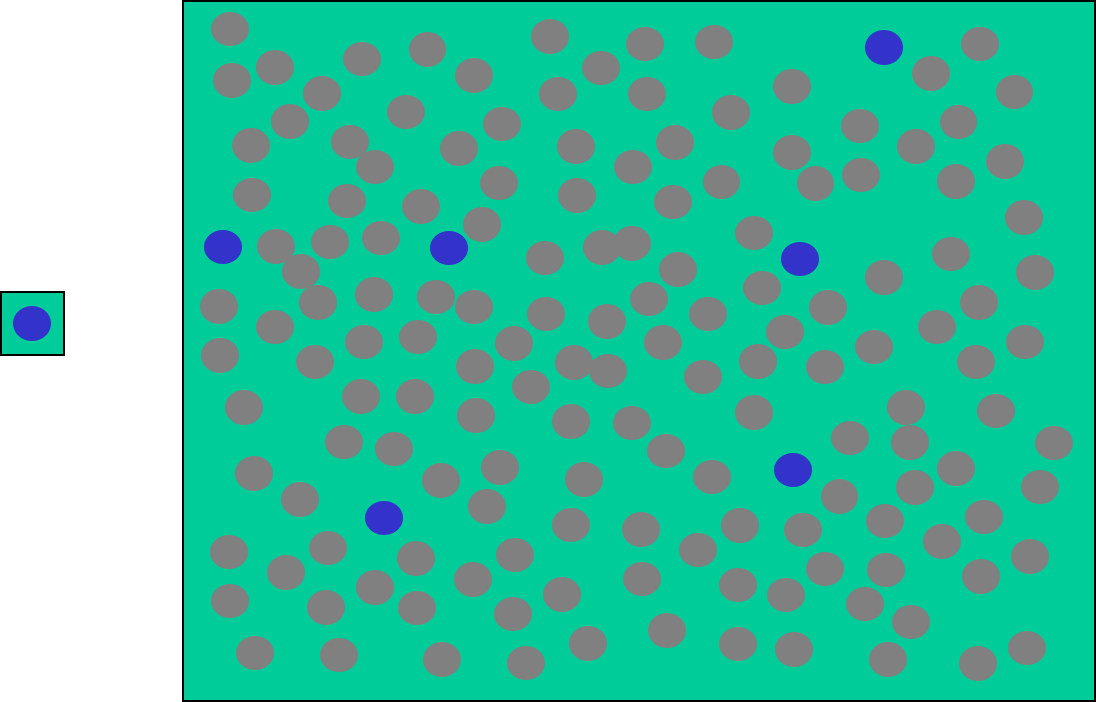
\includegraphics[scale=0.45]{10_Picture1.png}}}
    \end{picture}
    
\end{frame}



%Fer Andrei
%11
\definecolor{textalbastru}{RGB}{0,0,102}
\definecolor{fundal}{RGB}{255,255,255}
\setbeamercolor{background canvas}{bg=fundal}
\begin{frame}
{\textbf{Encoding color}}{\textcolor{red}{\rule{12cm}{1.2pt}}}

     \text{Common advice says use a ranibow scale}
     \begin{itemize}
     	\item[--] {Marcus, Murch, Healey}
        \item[--] {problems with rainbows}
     \end{itemize}
     
    \begin{picture}(0,0)
     \put(-10,-80){\hbox{
\includegraphics[scale=0.45]{11_Picture1.png}}}
    \end{picture}
    
    \vspace{200px}
    
\end{frame}



%Florică Cosmin
%15
\definecolor{fundal}{RGB}{255,255,255}
\definecolor{textalbastru}{RGB}{0,0,102}
\begin{frame}
{\textbf{Orientation}}{\textcolor{red}{\rule{12cm}{1.2pt}}}

    \begin{itemize}
    		\setlength\itemsep{1.6em}
     		\item[\checkmark]\textbf{{{selective}}}  
            \item[\checkmark]\textbf{{{associative}}}
            \item[$\neq$]\textbf{{{quantitative}}}
            \item[$\neq$]\textbf{{{order}}}
            \item[\checkmark]\textbf{{{length}}}
            \begin{itemize}
             \item[--]\hspace{10px}{\small{~5 in 2D; ? in 3D}}  
            \end{itemize}
            \begin{picture}(0,0)
         \put(105,145){\hbox{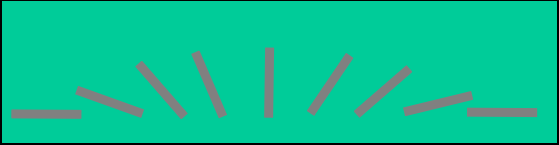
\includegraphics[scale=0.25]{15_Picture1.png}}}
         \put(105,105){\hbox{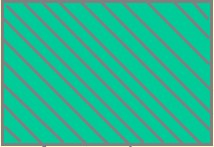
\includegraphics[scale=0.25]{15_Picture2.png}}}
         \put(160,105){\hbox{
\includegraphics[scale=0.25]{15_Picture3.png}}}
        \put(215,105){\hbox{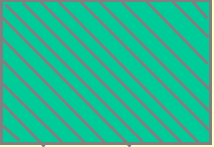
\includegraphics[scale=0.25]{15_Picture4.png}}}
        \put(90,60){\hbox{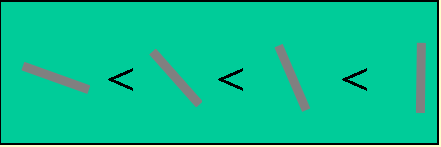
\includegraphics[scale=0.25]{15_Picture5.png}}}
        \put(190,60){\hbox{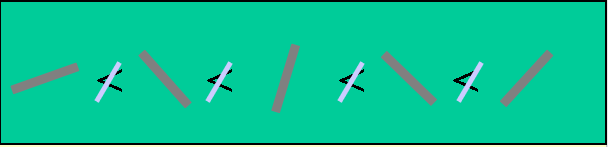
\includegraphics[scale=0.25]{15_Picture6.png}}}
         \put(177,63){\hbox{
\includegraphics[scale=0.75]{15_Picture7.png}}}
       \end{picture}
     \end{itemize}
\end{frame}



%Florică Cosmin
%16
\definecolor{fundal}{RGB}{255,255,255}
\definecolor{textalbastru}{RGB}{0,0,102}
\begin{frame}
{\textbf{Texture}}{\textcolor{red}{\rule{12cm}{1.2pt}}}

    \begin{itemize}
    		\setlength\itemsep{1.6em}        
     		\item[\checkmark]\textbf{{{selective}}}
            \item[\checkmark]\textbf{{{associative}}} 
            \item[$\neq$]\textbf{{{quantitative}}} 	
            \item[$\neq$]\textbf{{{order}}}
            \item[\checkmark]\textbf{{{length}}}
            \begin{itemize}
             \item[--]\hspace{10px}{\small{theoretically infinite}}  
            \end{itemize}
            \begin{picture}(0,0)
         \put(100,145){\hbox{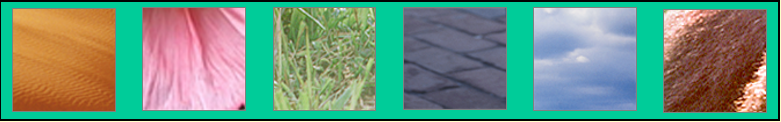
\includegraphics[scale=0.35]{16_Picture1.png}}}
         \put(100,105){\hbox{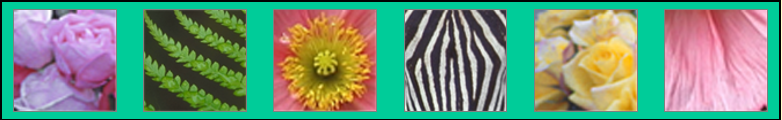
\includegraphics[scale=0.35]{16_Picture2.png}}}
         \put(100,45){\hbox{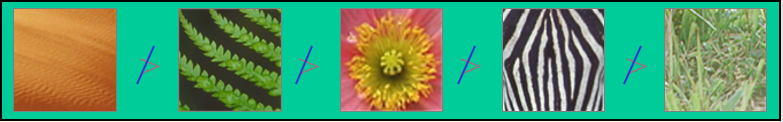
\includegraphics[scale=0.35]{16_Picture3.png}}}
       \end{picture}
     \end{itemize}
\end{frame}



%Florică Cosmin
%18
\definecolor{fundal}{RGB}{255,255,255}
\definecolor{textalbastru}{RGB}{0,0,102}
\begin{frame}
{\textbf{Motion}}{\textcolor{red}{\rule{12cm}{1.2pt}}}

    \begin{itemize}
    		\setlength\itemsep{1.6em}          
     		\item[\checkmark]\vspace{-5px}\textbf{{{selective}}}
            \begin{itemize}
             \item[--]\hspace{5px}{\small{motion is one of our most powerful attention grabbers}}
            \end{itemize}        
            \item[\checkmark]\vspace{-5px}\textbf{{{associative}}}
            \begin{itemize}
            \item[--]\hspace{5px}{\small{moving in unison groups objects effectively}}
            \end{itemize}          
            \item[$\neq$]\textbf{{{quantitative}}}
            \begin{itemize}
            \item[--]\hspace{5px}{\small{subjective perception}}
            \end{itemize}         		
            \item[$\neq$]\textbf{{{order}}}        
            \item[?]\textbf{{{length}}}
            \begin{itemize}
             \item[--]\hspace{10px}{\small{distinguishable types of motion?}}  
            \end{itemize}
     \end{itemize}
\end{frame}



%Florică Cosmin
%19
\definecolor{fundal}{RGB}{255,255,255}
\definecolor{textalbastru}{RGB}{0,0,102}
\begin{frame}
{\textbf{Motion}}{\textcolor{red}{\rule{12cm}{1.2pt}}}

\begin{figure}
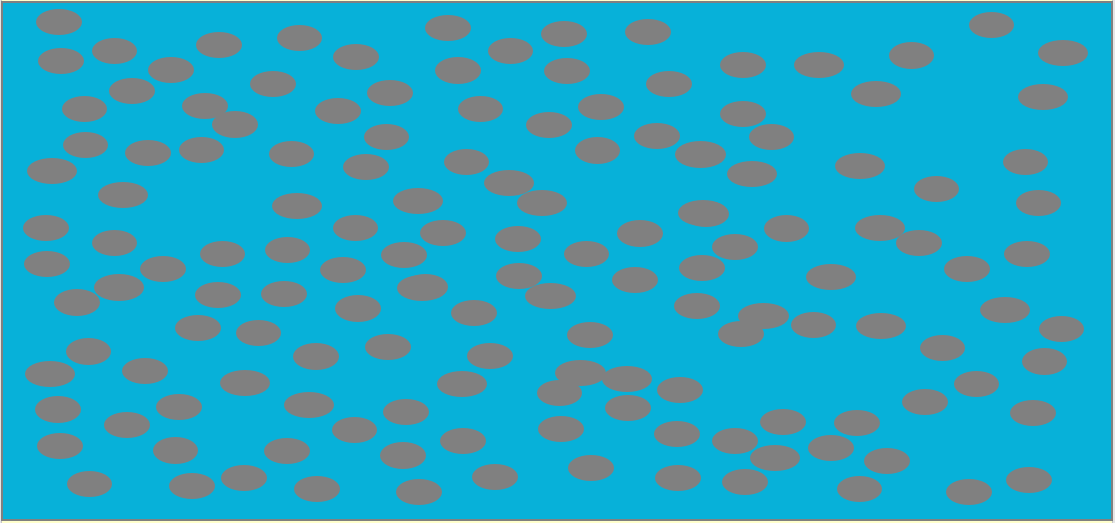
\includegraphics[scale=0.35]{19_Picture1.png}
\end{figure}

\end{frame}



%Florică Cosmin
%20
\definecolor{fundal}{RGB}{255,255,255}
\definecolor{textalbastru}{RGB}{0,0,102}
\begin{frame}
{\textbf{What you know now}}{\textcolor{red}{\rule{12cm}{1.2pt}}}

    \textbf{Attributes of visual variables}
    \begin{longtable}{ l p{3in} } 
		-- position & size \\
		-- shape & value\\
		-- orientation & color\\
		-- texture & motion\\
	\end{longtable}    
	
    \textbf{Characteristics of visual variables}
    \begin{longtable}{ l p{3in} } 
        -- selective \\
        -- associative \\
        -- quantitative \\
        -- order \\
        -- length \\
	\end{longtable}    
\end{frame}



{\setbeamercolor{background canvas}{bg=background}
\begin{frame}
{\textbf{*Bibliography}}{\textcolor{red}{\rule{12cm}{1.2pt}}}

        \begin{itemize}
        	\item[{$\bullet$}] Saul Greenberg, \textbf{Designing and building visual interfaces. Visual variables}, University of Calgary, Canada

        	\url{http://pages.cpsc.ucalgary.ca/~saul/481/}
			\newline

			
        	 
     	\end{itemize}
\end{frame}



\end{document}